\documentclass[a4paper, 12pt]{report}
\usepackage[italian]{babel}
\usepackage{lipsum}
\usepackage[none]{hyphenat}
\usepackage{geometry} 
\usepackage{ragged2e}
\usepackage{hyperref}
\usepackage{url}
\usepackage[dvipsnames]{xcolor}
\usepackage{float}
\usepackage{listings}
\usepackage{xcolor}
\usepackage{afterpage}
\usepackage[utf8]{inputenc}
\newcommand\blankpage{%
    \null
    \thispagestyle{empty}%
    \newpage}
\usepackage{multirow}
\definecolor{codegreen}{rgb}{0,0.6,0}
\definecolor{codegray}{rgb}{0.5,0.5,0.5}
\definecolor{codepurple}{rgb}{0.58,0,0.82}
\definecolor{backcolour}{rgb}{0.95,0.95,0.92}
\lstdefinestyle{mystyle}{
    backgroundcolor=\color{backcolour},   
    commentstyle=\color{codegreen},
    keywordstyle=\color{magenta},
    numberstyle=\tiny\color{codegray},
    stringstyle=\color{codepurple},
    basicstyle=\ttfamily\footnotesize,
    breakatwhitespace=false,         
    breaklines=true,                 
    captionpos=b,                    
    keepspaces=true,                 
    numbers=left,                    
    numbersep=5pt,                  
    showspaces=false,                
    showstringspaces=false,
    showtabs=false,                  
    tabsize=2
}

\lstset{style=mystyle, language=Python}

\newgeometry{
    top=3cm, 
    bottom=3cm, 
    outer=3cm,
    inner=3cm,
}
\usepackage{graphicx}
\graphicspath{immagini/}
\linespread{1.5}
\begin{document}
    \begin{titlepage}
        \begin{center}
	        \textsc{\Large {Università degli Studi di Napoli Parthenope\\}}
	        \vspace{0,7cm}
	        \textsc{\large {Dipartimento di Scienze e Tecnologie\\}}
	        \vspace{1cm}
	        
\includegraphics[width=0.32\textwidth]{immagini/logo.png}\\
	        \vspace{0,7cm}
	        \textsc{\large {Corso di laurea in informatica\\}}
	        \vspace{0,3cm}
	        \textsc{\large {Tesi di laurea\\}}
	        \vspace{1,4cm}
	        \textsc{\Large {RoboBVN: Assistive Robot for people’s language predictive of the later emergence of ASD\\}}
	        \vspace{2,5cm}
	    \end{center}
        \begin{minipage}[t]{.49\textwidth}
            \textbf{\large{Relatore}}\\
            \large{Prof.ssa Mariacarla Staffa}
            \vspace{0,7cm}
        \end{minipage}\hfill
        \begin{minipage}[t]{.49\textwidth}
            \hfill\textbf{\large{Candidato}}\\
            \hbox{}\hfill\large{Gianmarco Donnesi}\\
            \hbox{}\hfill\large{Matr. \scshape 0124002147}
        \end{minipage}
        \vspace{1,6cm}
	    {\begin{center}
	        \textsc{{Anno Accademico 2022/2023}}
	    \end{center}}
      \afterpage{\blankpage}
	\end{titlepage}
	\newpage
	\begin{flushright}
	\fontsize{12}{18}\selectfont{\textit{A Totò e Mimma, i miei nonni,}\\\textit{coloro che mi hanno insegnato }\\\textit{ad essere la persona che sono.}}
	\end{flushright}
    \afterpage{\blankpage}
    \fontsize{12}{18}\selectfont{\tableofcontents}
    \newpage
    \cleardoublepage
    \phantomsection
    \addcontentsline{toc}{chapter}{\listfigurename}
    \listoffigures
    \afterpage{\blankpage}
   
 \begin{sloppypar}
\chapter{Introduzione}
\fontsize{12}{19}\selectfont{
I disturbi dello spettro autistico (\textit{DSA}) si riferiscono a disturbi dello sviluppo neurologico con esordio nei primi tre anni di vita e sono caratterizzati  da  difficoltà  di  comunicazione, di interazione sociale e da modelli limitati e ripetitivi nei comportamenti, negli interessi  e nelle attività di un individuo.
 L’autismo  rappresenta  una sindrome molto complessa, nella maggior parte dei casi di natura genetica e poiché  le sue manifestazioni sono molto  varie  e  possono differire notevolmente da soggetto a soggetto, è  più appropriato  parlare  di  “spettro  autistico”.\newline
Per diversi anni i \textit{DSA} sono stati considerati essenzialmente rari con la prevalenza minore di un bambino affetto su mille. Ad oggi, il \textit{World Health Organization} stima che la prevalenza sia di un bambino su cento e sostiene che sembra essere in aumento negli anni futuri.
Essi vengono diagnosticati quando il soggetto, a seguito di test standardizzati somministrati individualmente, su lettura, calcolo, o espressione scritta, ottenga risultati significativamente al di sotto delle soglie predeterminate che tengono conto dell'età, dell'istruzione e del livello di intelligenza.\newline
Come confermato a più riprese dagli esperti, la diagnosi e l’avvio conseguente di un intervento precoce può migliorare notevolmente la prognosi dei bambini con DSA e la qualità di vita delle loro famiglie.
Purtroppo, la varietà e la diversità delle manifestazioni legate ai DSA, la limitata conoscenza degli stessi da parte delle famiglie, il numero insufficiente di centri specializzati e di professionisti esperti disponibili, concorrono a causare ritardi nella diagnosi e quindi nella cura.\newline
Le nuove tecnologie informatiche rispondono alla crescente esigenza di individuare le migliori pratiche per lo screening e la diagnosi dei DSA già nelle prime fasi dello sviluppo dell'individuo.
Esse, infatti, sono da tempo all’ attenzione del mondo medico, oltre che educativo e scientifico, per la valenza facilitante che possono avere nella progettazione di programmi abilitativi personalizzati/individualizzati \cite{Numero13}. 
In particolare, per i pazienti con DSA le tecnologie informatiche adeguatamente impiegate, costituiscono un valido supporto nei percorsi di intervento e di trattamento finalizzati al superamento dei deficit comunicativi e relazionali potenziando l’apprendimento, la comunicazione e la socializzazione.\newline
Esse consentono di usare un canale comunicativo prevalentemente visuo-spaziale, particolarmente adatto alle caratteristiche dei pazienti con disturbi dello spettro autistico. Inoltre, il linguaggio informatico, in quanto chiaro, strutturato e prevedibile, ha il grande pregio di non comportare inferenze emotive, incomprensibili per una persona con autismo.
Tra gli approcci più  innovativi vi è sicuramente quello relativo
alla possibilità  di utilizzare tecnologie assistive durante le sessioni di terapia. 
I rapidi progressi nell’area della robotica offrono oggi enormi possibilità di innovazione e di trattamento o addirittura di educazione per i pazienti affetti da DSA.
Fu lo scrittore ceco \textit{Karel Cˇapek}  che nel suo dramma fantascientifico 
teatrale \textit{R.U.R.} (\textit{I robot universali di Rossum}) nel 1920,  in  sostituzione  del  termine  “automa”,  ideò  il  termine “robot” che stava ad indicare una macchina meccanica con funzioni di lavoro. 
Successivamente, lo scrittore russo \textit{Isaac Asimov}  nel  1942  pubblicò   tre  leggi  ancor  oggi  geniali  nella loro intuizione. Si trattava delle tre leggi della robotica, nate per regolamentare e garantire il comportamento etico di una macchina dotata di intelligenza artificiale.\newline
All'epoca, tali leggi si limitavano ad apparire come l’acuta invenzione di uno scrittore di fantascienza. Oggi, invece, le ricerche scientifiche e tecnologiche hanno compiuto progressi tali da renderle quanto mai attuali; sono diventate un punto fermo della fantascienza e un fondamento dell’etica robotica.\newline
Da allora la robotica ha fatto dei progressi straordinari fino a  trasformare  gli  attuali  robot  in  entità autonome con capacità di movimento, apprendimento, comunicazione e adeguamento  all’ ambiente circostante,  fino  a  prospettare  la  possibilità  di  robot dotati di intelligenza artificiale (\textit{IA}).\newline
  La  robotica  di  assistenza  sociale (RAS) è quel campo della ricerca riguardante il modo in cui i robot assistono le persone attraverso l’interazione sociale. Essa costituisce un sottocampo dell’interazione uomo-robot (\textit{HRI}), volto allo sviluppo di interazioni efficienti con l’utente in contesti terapeutici  ed  educativi  per  aiutarlo  a  costruire  abilità  di  comportamento sociale \cite{Numero7}.\newline
L’utilizzo di interventi basati sulla RAS ha dimostrato in primo luogo il notevole potenziale nel trattamento dei DSA con l'aumento del coinvolgimento del paziente con difficoltà nella comunicazione. Inoltre, l'impiego di tali tecnologie ha messo a disposizione dei terapisti la possibilità di organizzare sessioni di trattamento più interattive \cite{Numero9}\cite{Numero10} con supporto negli aspetti valutativi (oggettivazione, raccolta dati), nonché la facoltà di delineare percorsi di cura riabilitativi innovativi e altamente personalizzati.
Il miglioramento ed il potenziamento dello sviluppo sociale, emotivo, cognitivo e sensoriale, sono i principali obiettivi terapeutici ed educativi per il trattamento e la cura dei DSA. Naturalmente, ognuna di queste aree richiede un approccio e tipologie di dispositivi specifici, per questo sono stati realizzati modelli di intervento distinti a seconda degli scopi della determinata competenza su cui lavorare.\newline
Nel contesto riabilitativo, le due categorie di robot che vengono maggiormente utilizzati sono quelli a scopo terapeutico e quelli a scopo assistivo. 
Nel presente lavoro di tesi, si è deciso di impiegare robot antropomorfi di tipo assistivo per favorire lo sviluppo di competenze emotive e sociali al fine di migliorare il benessere psicologico del paziente.\newline
Numerosi studi condotti su bambini affetti da disturbi dello spettro autistico hanno evidenziato risultati positivi in termini di interazione sociale.
I bambini hanno mostrato una maggiore interazione diadica e triadica,  uno sviluppo  migliore delle  capacità  di  comunicazione sociale e un’acquisizione di regole comportamentali più efficace.\newline 
Un robot umanoide è in grado di fornire gli stimoli sociali adeguati in modo molto simile a quello degli operatori umani, può essere riconosciuto facilmente come “compagno” e può essere programmato con applicazioni che sollecitano lo sviluppo di abilità interpersonali di cui i pazienti hanno bisogno: imitazione, contatto oculare e fisico, comunicazione verbale e non verbale. I robot possono attivare luci o musiche e compiono movimenti lenti e prevedibili al fine di fornire i rinforzi positivi di cui necessitano i pazienti.\newline
Allo stato attuale non esiste ancora un metodo esclusivo per confermare una diagnosi di autismo attraverso test di laboratorio, di neuroimaging o genetici; anche gli strumenti psicodiagnostici sono spesso difficili da impiegare per le difficoltà tipiche della sindrome. Rilevato che la diagnosi di autismo si basa in gran parte sulla valutazione clinica, l'avvalimento in fase diagnostica delle capacità del robot di rilevazione e registrazione delle risposte dell'individuo, consente di determinare con una certa accuratezza l'eventuale presenza di un paziente affetto da DSA.\newline
Le valutazioni sono favorite fornendo stimoli standardizzati per valutare i comportamenti caratteristici dell’autismo così da giungere a diagnosi integrate sempre più affidabili. 
La risposta del paziente agli stimoli del robot umanoide, al tono della sua voce, ai movimenti degli occhi, ai cambiamenti di espressione e al tipo di conversazione forma dati che vengono raccolti ed elaborati per una successiva analisi. Quest'ultima viene svolta da un lato in maniera totalmente automatizzata e dall'altro tramite una valutazione clinica di un esperto.\newline
Tutte le considerazioni e le ricerche sopra esposte hanno posto le basi per il presente lavoro di tesi, il quale ha avuto come obiettivo lo sviluppo di una applicazione RAS per la somministrazione di test per l’analisi delle funzioni cognitivo-linguistiche in individui affetti da disturbi dello spettro autistico \cite{Numero11}.
}
 \end{sloppypar}
 \afterpage{\blankpage}
\begin{sloppypar}
\chapter{Tecnologie impiegate}
\fontsize{12}{19}\selectfont{
In questo capitolo sono descritte in dettaglio le tecnologie utilizzate per la realizzazione dell'applicazione. 
Lo studio di esse ha occupato una parte rilevante del lavoro di tesi in quanto si tratta di tecnologie di nuova generazione, come di seguito elencate:
\vspace{0.2cm}
\begin{enumerate}
    \item  \textbf{Pepper}: robot umanoide progettato e sviluppato dall'azienda \textit{SoftBank Robotics}\texttrademark, specializzata nella progettazione, sviluppo e commercializzazione di robot umanoidi e servizi robotici intelligenti.
\vspace{0.3cm}
\item  \textbf{Choregraphe}: software sviluppato dall'azienda \textit{SoftBank Robotics}\texttrademark, progettato specificamente
per la programmazione e la gestione dei robot umanoidi della
famiglia \textit{NAO}, compresi \textit{NAO} e \textit{Pepper}.
\vspace{0.3cm}
\item \textbf{NAOqi OS}: un sistema operativo sviluppato da\textit{ SoftBank Robotics}\texttrademark, che fornisce
un’interfaccia di programmazione completa e potente, per accedere e
controllare le funzionalità dei robot della famiglia \textit{NAO}.
\end{enumerate}
\begin{figure}[H]
\centering

\includegraphics[width=0.65\textwidth]{immagini/softbank.png}
\caption{Logo dell'azienda SoftBank Robotics}
\end{figure}
\vspace{0.4cm}
}
\section{Pepper}
\fontsize{12}{19}\selectfont{Pepper è un robot umanoide progettato e sviluppato dall'azienda SoftBank Robotics\texttrademark,
un’azienda specializzata nella creazione di robot sociali \cite{NAO}. Ha un’altezza di circa 1
metro e 20 cm, un peso di circa 30 kg e presenta un design in grado di conferirgli
sembianze umane. Esso è alimentato da un sistema operativo basato su \textit{Linux} e utilizza una
combinazione di software proprietari e applicazioni sviluppate da terze parti per
fornire una vasta gamma di funzionalità. 
È stato progettato per svolgere compiti
come l’assistenza all’utente, la presentazione di informazioni, l’intrattenimento
e l’interazione sociale. 
\newline
L’obiettivo principale del suo utilizzo è quello di creare
connessione emotiva con l’utente, offrendo un’esperienza coinvolgente e personalizzata.
\vspace{1cm}
\begin{figure}[H]
\centering
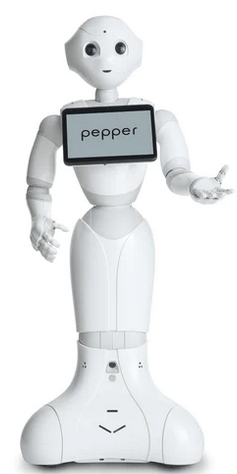
\includegraphics[width=0.33\textwidth]{immagini/pepper1.png}
\caption{Robot umanoide Pepper}
\end{figure}
\vspace{1cm}
Pepper è costituito da un sistema a tre strati.
\newline
La testa contiene tutti i sensori e i componenti di elaborazione dei dati, compresi microfoni, telecamere, sensori di prossimità e un processore \textit{Intel \textsuperscript{\textregistered} Atom\texttrademark}. 
\newline
Il torace ospita il computer principale, che include una \textit{CPU}, una \textit{GPU}, memoria \textit{RAM} e \textit{flash}, nonché connettività \textit{Wi-Fi} e \textit{Ethernet} per consentire il collegamento a Internet e l'accesso a informazioni e servizi basati sul cloud.
\newline
La base contiene le ruote per la mobilità del robot, la batteria per l'alimentazione e sonar per l'individuazione di ostacoli durante lo spostamento del robot.
\newline
L'androide è equipaggiato con un vasto assortimento di sensori,
tra cui telecamere, microfoni direzionali, sensori di prossimità e sensori tattili, che
gli consentono di percepire l’ambiente circostante e interagire in modo intelligente
con le persone. 
\newline
Questi vengono elencati ed analizzati di seguito:
\vspace{0.3cm}
\begin{itemize}
   \item \textbf{Sensori di contatto}: situati nelle mani e nelle dita, consentono a Pepper di rilevare il tocco e le interazioni fisiche.
   \vspace{0.3cm}
   \item \textbf{Sensori di prossimità}: posizionati nel petto, rilevano la presenza di oggetti o persone nelle vicinanze.
   \vspace{0.3cm}
   \item \textbf{Sensori a infrarossi}: consentono a Pepper di misurare la distanza dagli oggetti e di eluderli per evitare collisioni.
   \vspace{0.25cm}
   \item \textbf{Microfoni}: permettono al robot di rilevare e registrare i suoni ambientali.
   \vspace{0.3cm}
   \item \textbf{Telecamere}: Pepper ha telecamere ad alta definizione posizionate nella testa e nel petto per riconoscere i volti, rilevare le espressioni facciali e percepire l'ambiente visivo.
   \vspace{0.3cm}
\end{itemize}
Il robot utilizza una combinazione di ruote e giunti per il movimento. Ha ruote omnidirezionali nella base che gli consentono di ruotare in ogni direzione in modo fluido. Inoltre l'automa è equipaggiato con un sistema di riconoscimento vocale avanzato che gli consente di comprendere e rispondere a comandi vocali in diverse lingue. Ancora, è in grado di analizzare il linguaggio naturale utilizzando algoritmi di elaborazione del linguaggio e di generare risposte coerenti.
\newline
Pepper utilizza il framework NAOqi, basato su Linux, che fornisce un'ampia gamma di API e strumenti per gli sviluppatori per creare applicazioni personalizzate e ampliare le capacità del robot.\newline
Gli sviluppatori possono creare moduli comportamentali, implementare algoritmi di visione artificiale, elaborare dati sensoriali e personalizzare l'interazione con l'utente.
Infine, Pepper presenta un display touch da 10,1 pollici montato sul petto. Questo schermo viene utilizzato per visualizzare informazioni e comunicare con l'utente tramite interfacce personalizzate.
\newline
In conclusione, la sua versatilità, la sua tecnologia innovativa e la capacità
di interazione \textit{user-friendly} lo hanno reso sicuramente un prezioso e interessante
strumento, offrendo opportunità
di apprendimento e di sperimentazione nelle nuove frontiere della robotica e
dell’intelligenza artificiale.
}
\section{Choregraphe}
\fontsize{12}{19}\selectfont{Aldebaran Choregraphe \cite{Aldebaran} è un ambiente di programmazione visuale utilizzato
per creare e gestire comportamenti di robot umanoidi della famiglia NAO, messo
a disposizione dalla SoftBank Robotics. 
\vspace{1cm}
\begin{figure}[H]
\centering
\includegraphics[width=0.5\textwidth]{immagini/choregraphe.png}
\caption{Logo del software Aldebaran Choregraphe}
\end{figure}
\vspace{1cm}



Esso offre un ambiente di sviluppo
basato su un’interfaccia grafica intuitiva, che permette agli sviluppatori di programmare
i robot utilizzando il concetto di "grafi di comportamento". Questi
grafi rappresentano una serie di azioni, movimenti e interazioni che il robot può
eseguire. I comportamenti possono essere creati collegando blocchi funzionali predefiniti,
chiamati \textit{"box"}, tramite linee di connessione che rappresentano il flusso
dell’esecuzione delle azioni del robot.\newline Ogni box rappresenta una specifica azione o una sequenza di azioni che il
robot può compiere, come ad esempio camminare, riconoscere il volto umano o
riprodurre un suono.\newline
Choregraphe fornisce anche una vasta gamma di strumenti per la personalizzazione
dei comportamenti dei robot. Infatti tramite l’utilizzo di script Python
all’interno del software, è possibile estendere le funzionalità di base dei box predefiniti o creare nuovi box personalizzati.\newline Sono messi a disposizione dello sviluppatore anche strumenti di simulazione (\textit{virtual robot}) che consentono di testare i comportamenti dei robot senza doverli eseguire fisicamente. Ciò facilita il processo di debugging e di ottimizzazione delle sequenze di azioni sviluppate.
\vspace{1cm}
\begin{figure}[H]
\centering
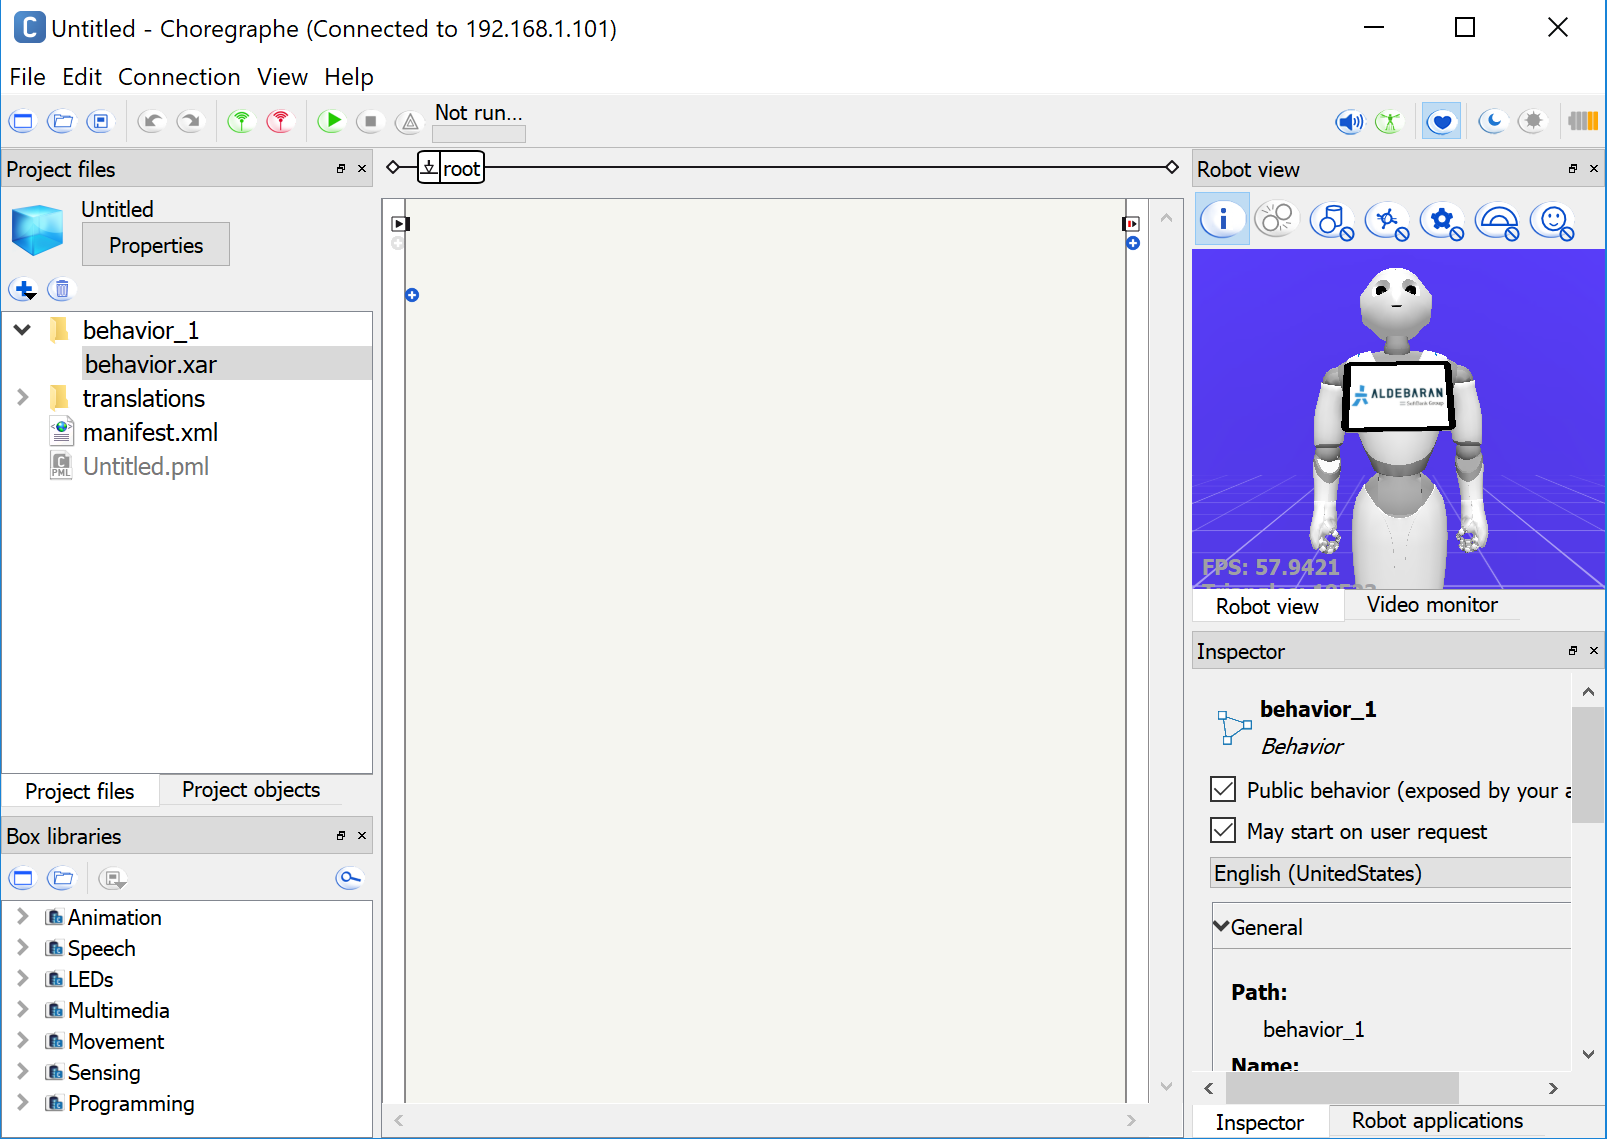
\includegraphics[width=1\textwidth]{immagini/Choregraphe.png}
\caption{Interfaccia del software Aldebaran Choregraphe}
\end{figure}
\vspace{1cm}
Il software si basa su un’architettura di tipo \textit{client-server}, in cui l’interfaccia
utente e l’elaborazione dei comportamenti avvengono su un computer (\textit{client}) e le
istruzioni vengono inviate al robot (\textit{server}) per l’esecuzione.\newline Per comunicare con
il robot, Choregraphe utilizza un protocollo di comunicazione che consente di accedere alle funzionalità
hardware dell'automa, come i sensori, i motori e i moduli di intelligenza artificiale,
attraverso un’API completa e ben documentata. Questo permette agli sviluppatori
di integrare facilmente i comportamenti creati con Choregraphe con altre
applicazioni e sistemi come ad esempio \textit{ROS} (Robot Operating Sistem), framework \textit{open-source} utilizzato per lo sviluppo di applicazioni robotiche.\newline In conclusione, l’intero ambiente di sviluppo si è rivelato essere un potente ed intuitivo
strumento di programmazione visuale facilmente adattabile anche all’ implementazione
di comportamenti più complessi, creando esperienze interattive e coinvolgenti per gli utenti.
}
\newpage

\section{NAOqi OS}
\fontsize{12}{19}\selectfont{
NAOqi OS è un sistema operativo sviluppato da \textit{SoftBank Robotics} per i loro robot umanoidi NAO e Pepper. Si tratta di una distribuzione GNU/Linux basata su Gentoo\footnote{\textbf{Gentoo}: distribuzione Linux basata su sorgenti, che si distingue per il suo approccio altamente personalizzabile e orientato alle prestazioni.} e sviluppata appositamente per le esigenze degli automi dell'azienda \textit{Aldebaran}.
\vspace{1cm}
\begin{figure}[H]
\centering

\includegraphics[width=0.48\textwidth]{immagini/naoqi.png}
\caption{Logo di NAOqi OS}
\end{figure}
\vspace{1cm}
La particolarità di questo sistema operativo si ritrova nella sua architettura a componenti modulari. Ogni componente, chiamato "\textit{module}", svolge un compito specifico, come il controllo del movimento, la percezione dei sensori o l'elaborazione del linguaggio naturale.\newline Questi moduli interagiscono tra loro attraverso un sistema di messaggistica per consentire la comunicazione e la cooperazione.\newline NAOqi OS utilizza un middleware chiamato "\textit{ALBroker}" per gestire la comunicazione tra i moduli. L'\textit{ALBroker} funge da intermediario tra i moduli, consentendo loro di pubblicare e sottoscriversi a \textit{topic}, inviare e ricevere messaggi, e richiedere e fornire servizi.
\vspace{0.7cm}
\begin{flushleft}
\textbf{Topic}
\end{flushleft}
Più nello specifico, con \textit{topic} si intende un canale di comunicazione asincrona utilizzato per scambiare messaggi tra i diversi componenti di un sistema robotico.\newline Un topic può essere considerato come un argomento di discussione su cui i nodi del sistema possono pubblicare e sottoscriversi per inviare e ricevere messaggi relativi a quell'argomento specifico.
\begin{figure}[H]
\centering
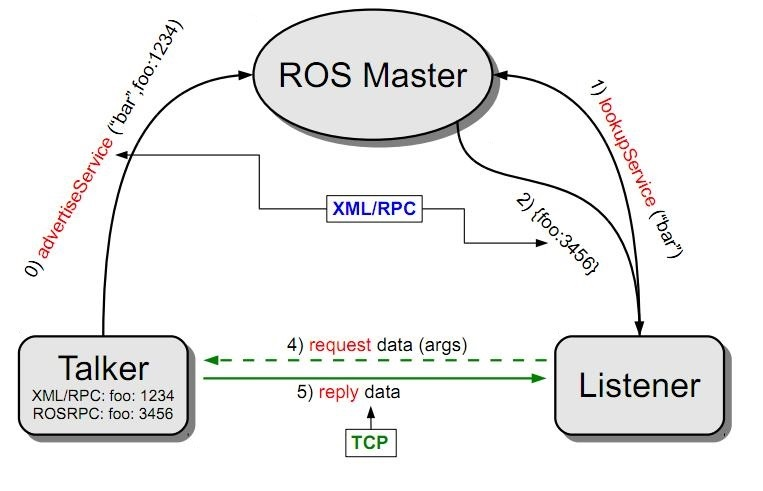
\includegraphics[width=0.88\textwidth]{immagini/comunicazione_ros.png}
\caption{Esempio di comunicazione tra i nodi in ROS}
\end{figure}
\vspace{1cm}
I messaggi possono contenere dati di vario tipo, come informazioni provenienti dai sensori del robot, comandi di controllo, dati di stato, immagini, odometria (consente di stimare e tenere traccia della posizione e dell'orientamento di un robot in base alle informazioni dei suoi motori di movimento) e altro ancora.

 Quando un nodo pubblica un messaggio su un topic, tutti i nodi che si sono sottoscritti a quel topic riceveranno il messaggio e potranno elaborarlo di conseguenza. Ciò consente una comunicazione efficiente e disaccoppiata tra i diversi componenti del sistema robotico, in quanto i nodi possono inviare e ricevere dati senza la necessità di un collegamento diretto uno-a-uno.\vspace{1.5cm}\newline 
 Tornando a NAOqi OS, questo offre una serie di strumenti di sviluppo per facilitare la creazione di applicazioni robotiche. Questi strumenti includono l'ambiente di programmazione visuale Choregraphe, che consente di creare comportamenti per il robot trascinando e rilasciando blocchi di azioni, e l'API di sviluppo NAOqi SDK, che fornisce una vasta gamma di funzioni per interagire con i moduli e controllare il robot.\newline
 \vspace{0.3cm}
 Queste funzioni vengono descritte di seguito:
 \vspace{0.1cm}
 \begin{itemize}
     \item \textbf{Accesso ai sensori}: fornisce un’interfaccia per accedere ai
sensori del robot, come telecamere, microfoni, sensori tattili e giroscopi. Si
possono utilizzare queste informazioni sensoriali per creare comportamenti
basati sulla percezione dell’ambiente circostante.
\vspace{0.5cm}
     \item \textbf{Controllo dei motori}: permette di controllare i motori del robot,
consentendo di gestire il movimento e la postura degli attuatori. Ciò consente
di creare movimenti fluidi e naturali per i robot umanoidi.
\vspace{0.5cm}
     \item \textbf{Gestione del suono}: offre funzionalità per la registrazione e
la riproduzione dei suoni, consentendo ai robot di comunicare e interagire
tramite l’emissione di suoni o la riproduzione di file audio predefiniti.
\vspace{0.5cm}
     \item \textbf{Riconoscimento vocale e linguaggio naturale}: sono inclusi moduli
per il riconoscimento e la sintesi vocale, consentendo ai robot
di comprendere e rispondere ai comandi vocali generando feedback
verbali.
\vspace{0.5cm}
     \item \textbf{Intelligenza artificiale}: sono integrati moduli di intelligenza artificiale,
come il riconoscimento facciale e il riconoscimento degli oggetti, che consentono
ai robot di interagire con gli esseri umani e di analizzare l’ambiente
circostante.
\vspace{0.4cm}
     \item \textbf{Comunicazione}: è supportata la comunicazione tra i robot stessi
o con dispositivi esterni attraverso protocolli come TCP/IP, permettendo
la collaborazione tra più robot o l’integrazione con altri sistemi.
 \end{itemize}
\vspace{1.5cm}
Per concludere, questo sistema operativo embedded\footnote{\textbf{Sistema operativo embedded}: sistema operativo ottimizzato per funzionare su hardware a risorse limitate, con restrizioni di memoria, potenza di calcolo e spazio di archiviazione. Caratterizzato da un basso consumo energetico, affidabilità e una richiesta minima di risorse di sistema rispetto alle distribuzioni \textit{desktop} o \textit{server}.} è progettato per essere multi-piattaforma, per semplificare lo sviluppo di applicazioni robotiche e gestire
comportamenti personalizzati, consentendo agli sviluppatori di concentrarsi
sulla logica dell’applicazione senza doversi preoccupare dei dettagli implementativi
e tecnici di basso livello.
}
\newpage
\end{sloppypar}
\afterpage{\blankpage}
 \begin{sloppypar}
\chapter{Applicazione Realizzata}
\fontsize{12}{19}\selectfont{Questo capitolo ha lo scopo di descrivere ed analizzare l’applicazione sviluppata per questo lavoro di tesi per il training di pazienti affetti da disturbi dello spettro autistico (DSA) e caratterizzata dalle potenzialità e risorse offerte dalle tecnologie introdotte nel capitolo precedente.\newline
In particolare, per \textit{training} si intende un insieme di attività volte al potenziamento delle abilità cognitive di un individuo\cite{Numero14}. Esse richiedono un serio e attento processo multidisciplinare che coinvolge diversi professionisti del settore medico e terapeutico, il cui obiettivo principale è valutare le abilità cognitive, comportamentali e sociali dei pazienti al fine di fornire una diagnosi accurata e un piano di trattamento personalizzato.\newline Inizialmente viene effettuata una valutazione da un team di specialisti che includono psicologi, psichiatri, neuropsichiatri infantili e terapisti occupazionali. Questa fase permette di raccogliere informazioni dettagliate sullo sviluppo del paziente, le sue abilità cognitive, il linguaggio, il comportamento sociale e le competenze motorie.\newline Sulla base delle informazioni raccolte nella valutazione iniziale, vengono selezionati i test più appropriati da sottoporre al paziente.\newline Questi test possono includere valutazioni standardizzate che misurano le abilità cognitive, il linguaggio, le abilità sociali e il comportamento adattivo dell'individuo.\newline

Nello specifico sono stati realizzati ed implementati due test molto diffusi per il training di pazienti affetti da DSA:
\begin{itemize}
\vspace{0.7cm}
    \item \textbf{Test sulla Discriminazione uditiva}\newline
    Il test sulla discriminazione uditiva è un test per l’analisi  delle funzioni linguistiche del paziente;
\vspace{1.2cm}
    \item \textbf{Test della Torre di Londra (TOL)}\newline
    Il Test della Torre di Londra (TOL) è un test per l’analisi delle funzioni esecutive del paziente.
\end{itemize}
\begin{figure}[H]
\centering
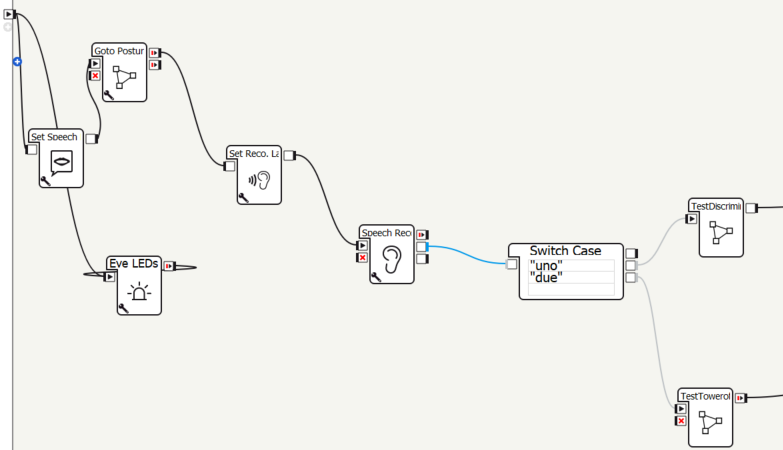
\includegraphics[width=1\textwidth]{immagini/applicazione.png}
\caption{Panoramica dell' applicazione realizzata tramite  il software Choregraphe}
\end{figure}
}

\newpage
\section{Discriminazione uditiva}
\fontsize{12}{19}\selectfont{La discriminazione uditiva è la capacità di percepire e riconoscere, attraverso
l’udito, le caratteristiche che rendono diversi fra loro i suoni della propria lingua, e
di attribuire ad essi un significato. Infatti, ogni fonema (ovvero ogni suono della
lingua) si differenzia dagli altri per una o più caratteristiche, definite “tratti”.\newline
Molte condizioni, tra cui l’autismo, possono influenzare l’abilità dell’individuo di
ascoltare e capire ciò che sente, ossia di comprendere, confrontare e distinguere i
“suoni” del linguaggio parlato.\newline Il Test sulla Discriminazione uditiva di \textit{Pinton}
e \textit{Zanettin} (1998) è utilizzato per valutare le abilità uditive e di elaborazione del
suono in individui con disturbi dello spettro autistico.
Nel caso particolare questo test è stato adoperato per valutare la capacità
uditiva dell’individuo di distinguere tra coppie di \textit{non parole}.\newline
La prova è composta
da 37 item, ciascuno dei quali rappresenta una coppia di non parole da
discriminare. Per ogni coppia vengono comunicate le non parole al paziente, il quale ha il compito di riconoscere se queste risultano essere uguali o diverse tra loro.\newline
Nel caso in cui
la risposta fosse corretta, questo comporterebbe un aumento del punteggio del
paziente (definito \textit{score} e registrato per ogni paziente). Lo score di ogni paziente rappresenta
una metrica fondamentale per il terapista, il quale dopo averlo analizzato
può verificare la presenza di eventuali disturbi nelle funzionalità uditive del paziente.
}
\vspace{0.2cm}
\subsection{Implementazione}
\fontsize{12}{19}\selectfont{Per l’implementazione di questo test sono stati utilizzati diversi box script Python in Choregraphe, i quali verranno analizzati di seguito:
\vspace{0.4cm}
\begin{itemize}
    \item \textbf{Animated Say text}: box che consente a Pepper di emettere messaggi
vocali animati. Questo box integra le funzionalità di sintesi vocale del robot,
consentendogli di comunicare verbalmente con gli utenti in modo coinvolgente e
realistico. Riceve in input un box testuale e lo trasforma in un messaggio vocale
animato.
\vspace{0.3cm}
\begin{figure}[H]
\centering
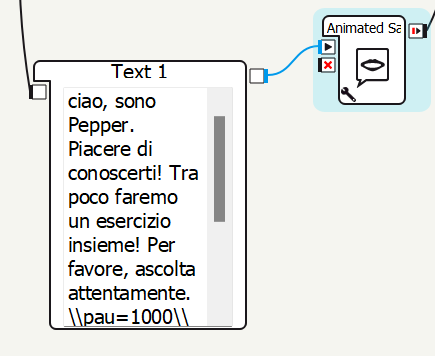
\includegraphics[width=0.5\textwidth]{immagini/Text.png}
\caption{Box per la lettura di testo animato}
\end{figure}
\vspace{0.3cm}
    \item \textbf{Record Sound}: box che permette di registrare i suoni catturati dai microfoni
direzionali di Pepper e salvarli sulla memoria temporanea di quest’ultimo.
\vspace{0.3cm}
\begin{figure}[H]
\centering
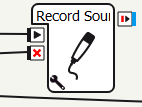
\includegraphics[width=0.23\textwidth]{immagini/RS.png}
\caption{Box per la registrazione audio}
\end{figure}
\vspace{0.3cm}    
    \item \textbf{Record Video}: box che permette di registrare video catturati dalle telecamere
frontali posizionate negli occhi di Pepper e salvarlo sulla memoria temporanea
di quest’ultimo.
\vspace{0.1cm}
\begin{figure}[H]
\centering
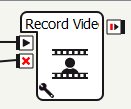
\includegraphics[width=0.23\textwidth]{immagini/RV.png}
\caption{Box per la registrazione video}
\end{figure}
\vspace{0.3cm}    
    \item \textbf{Face Tracker}: box progettato per rilevare e tracciare i volti umani
nell’ambiente circostante il robot. Questo modulo consente a Pepper di identificare
e seguire i volti umani, facilitando l’interazione e la comunicazione
con gli utenti. Questo modulo utilizza una combinazione di algoritmi di visione
artificiale e sensori per individuare i volti presenti nell’ambiente circostante.\newline L’immagine acquisita
viene quindi elaborata utilizzando algoritmi di elaborazione dell’immagine
per individuare le caratteristiche facciali comuni associate ai volti umani, come
gli occhi, il naso e la bocca. Questa elaborazione può includere tecniche come
la segmentazione dell’immagine, la rilevazione dei contorni e il riconoscimento
delle caratteristiche.\newline
Una volta individuato il volto, il modulo Face Tracker traccia
e segue i movimenti di quest’ ultimo nel tempo. Questo consente a Pepper
di mantenere una connessione visiva con le persone nell’ambiente e di rilevare
eventuali cambiamenti di posizione o espressione facciale. Il robot quindi può
mantenere il contatto visivo con una persona mentre si sposta o può indirizzare i
suoi movimenti e le sue espressioni facciali verso un individuo specifico per creare
una connessione personale.
\vspace{0.1cm}
\begin{figure}[H]
\centering
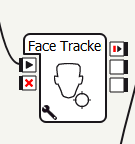
\includegraphics[width=0.23\textwidth]{immagini/FT.png}
\caption{Box per il tracciamento del volto umano}
\end{figure}
\vspace{0.3cm}      
    \item \textbf{Set Language}: box che permette di settare la lingua riconosciuta e parlata
del robot.
\vspace{0.1cm}
\begin{figure}[H]
\centering
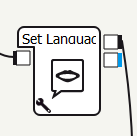
\includegraphics[width=0.23\textwidth]{immagini/Language.png}
\caption{Box per settare la lingua riconosciuta dal robot}
\end{figure}
\vspace{0.3cm}       
    \item \textbf{LRS} (lettura,riconoscimento vocale e incremento dello score): box che
racchiude uno script python personalizzato e che permette al robot di leggere le
coppie di non parole all’utente, aspettare la risposta di quest’ ultimo e verificarne
la correttezza. Nel caso in cui la risposta fosse corretta, verrebbe incrementato lo
score dell’utente, salvando il valore di quest’ ultimo in un file esterno.
\vspace{0.1cm}
\begin{figure}[H]
\centering
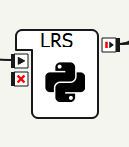
\includegraphics[width=0.23\textwidth]{immagini/LRS.png}
\caption{Box Python personalizzato}
\end{figure}
\vspace{0.3cm} 
\end{itemize}
Di seguito viene riportato e analizzato il codice dello script Python personalizzato denominato
LRS:
\begin{figure}[H]
\centering
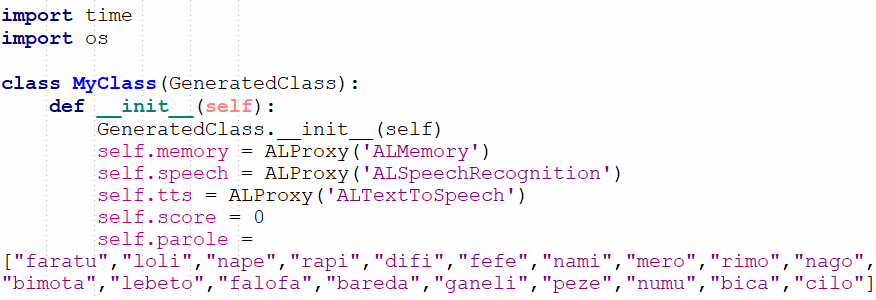
\includegraphics[width=1\textwidth]{immagini/lrs1.png}
\end{figure}
Alla creazione della classe vengono inizializzati gli oggetti che verranno utilizzati
per accedere alla memoria tramite modulo \textit{ALMemory}, al riconoscimento della
voce umana tramite modulo \textit{ALSpeechRecognition} e per la lettura vocale di un
testo tramite modulo \textit{ALTextToSpeech}. Fatto ciò viene inizializzata la lista delle
non parole che faranno parte del test.
\vspace{0.3cm}
\begin{figure}[H]
\centering

\includegraphics[width=0.7\textwidth]{immagini/lrs2.png}
\end{figure}
\vspace{0.3cm}
La funzione \textit{onLoad} viene invocata al caricamento del box e permette di inizializzare
alcuni parametri del robot. Viene impostata la lingua del componente
di sintesi vocale (\textit{self.speech}) su italiano e viene settato il parametro di velocità
(\textit{speed}) del componente di sintesi vocale (\textit{self.tts}) che rappresenta la velocità di
lettura di un testo di Pepper.
\vspace{0.3cm}
\begin{figure}[H]
\centering
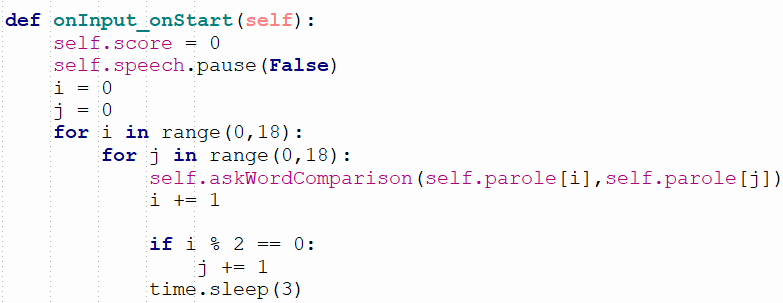
\includegraphics[width=1.05\textwidth]{immagini/lrs3.png}
\end{figure}
\vspace{0.3cm}
La funzione \textit{onInput onStart} viene invocata quando il box riceve un input esterno.
In particolare il funzionamento di questa porzione di codice viene descritto di
seguito.
\newline
Per prima cosa viene inizializzata a 0 una variabile \textit{score} che terrà traccia
del punteggio del paziente durante il test. Successivamente viene richiamata l’esecuzione del
componente di sintesi vocale e vengono inizializzati due indici, \textit{i} e \textit{j}, per riferirsi di
volta in volta a due non parole dalla lista di non parole inizializzata in precedenza.\newline
Il ciclo \textit{for} successivo permette di iterare, scorrendo la lista di non parole e creando
delle coppie da comunicare al paziente per lo svolgimento del test.\newline
A questo punto viene richiamata la funzione \textit{askWordComparison} il cui funzionamento
verrà analizzato successivamente. Al termine della funzione viene
utilizzato il metodo \textit{time.sleep()} per introdurre un ritardo di 3 secondi nel programma,
così da creare una pausa tra le iterazioni del ciclo.
\begin{figure}[H]
\centering
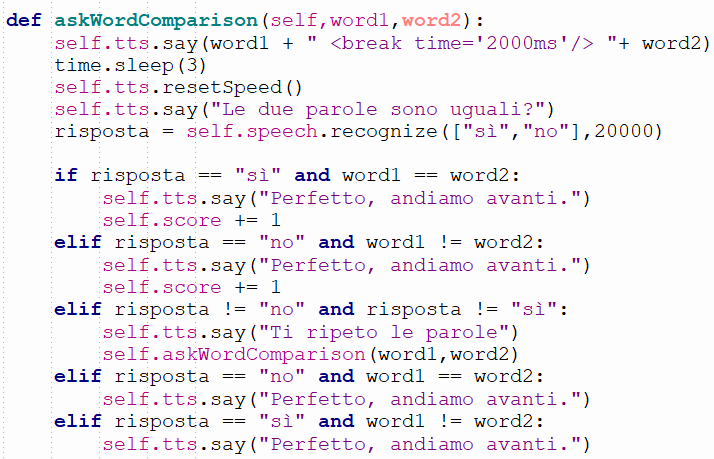
\includegraphics[width=1\textwidth]{immagini/lrs4.png}
\end{figure}
\vspace{0.3cm}
La funzione \textit{askWordComparison} prende in input due parole (\textit{word1} e \textit{word2}) e
svolge una serie di operazioni per confrontare la risposta del paziente, dopo averle
comunicate a quest’ultimo.\newline
Per prima cosa viene utilizzo il componente di sintesi vocale (\textit{self.tts}) per
riprodurre l’audio delle due non parole concatenate insieme, separandole da una pausa
di 2000 millisecondi (2 secondi). Viene utilizzato il metodo \textit{say} facendo si che
Pepper pronunci le due non parole, separate da una pausa per scandirle correttamente,
al paziente.\newline
Fatto ciò Pepper porrà una domanda al paziente, chiedendo se le due
non parole siano uguali e resterà in attesa di una sua risposta.\newline
Una volta ottenuta verrà analizzata per 5 casistiche:
\vspace{0.2cm}
\begin{enumerate}
    \item Se la risposta dell’utente è "\textbf{sì}" e le due parole sono \textbf{uguali}, viene incrementato
il punteggio del paziente in quanto la risposta risulta corretta e viene
pronunciato il messaggio "\textit{Perfetto, andiamo avanti.}"
\vspace{0.2cm}
\item Se la risposta dell’utente è "\textbf{no}" e le due parole sono \textbf{diverse}, viene incrementato
il punteggio del paziente in quanto la risposta risulta corretta e
viene pronunciato il messaggio "\textit{Perfetto, andiamo avanti.}"
\vspace{0.2cm}
\item Se la risposta dell’utente non è né "\textbf{no}" né "\textbf{sì}", viene pronunciato il messaggio
"\textit{Ti ripeto le parole}" e la funzione \textit{askWordComparison} viene richiamata nuovamente per ottenere una nuova risposta dall’utente.
\vspace{0.2cm}
\item Se la risposta dell’utente è "\textbf{no}" e le due parole sono \textbf{uguali}, non viene
incrementato il punteggio del paziente in quanto la risposta non è corretta
e viene pronunciato il messaggio "\textit{Perfetto, andiamo avanti.}"
\vspace{0.2cm}
\item Se la risposta dell’utente è "\textbf{sì}" e le due parole sono \textbf{diverse}, non viene
incrementato il punteggio del paziente in quanto la risposta non è corretta
e viene pronunciato il messaggio "\textit{Perfetto, andiamo avanti.}"
\end{enumerate}
\vspace{0.3cm}
\begin{figure}[H]
\centering

\includegraphics[width=0.8\textwidth]{immagini/lrs5.png}
\end{figure}
\vspace{0.3cm}
La funzione \textit{saveScore} accetta due argomenti: \textbf{score}, che rappresenta il punteggio
del paziente da salvare e \textbf{filepath}, che indica il percorso del file in cui il punteggio
verrà salvato.\newline
Più nello specifico, la funzione accede al file specificato dal \textbf{filepath} passato
come argomento, crea una stringa formattata che include il punteggio e scrive
questa stringa all’interno del file.
\vspace{0.3cm}
\begin{figure}[H]
\centering

\includegraphics[width=1\textwidth]{immagini/lrs6.png}
\end{figure}
\vspace{0.3cm}
Al termine dello script viene invocata la procedura \textit{onInput onStop} che si occupa
di attivare l’output del box, di richiamare la funzione \textit{saveScore} per salvare il
punteggio del paziente su un file esterno e di inizializzare il valore della variabile
\textit{score} a 0.
}
\newpage




\section{Torre di Londra (ToL)}
\fontsize{12}{19}\selectfont{
Il Test della Torre di Londra (ToL) è un test cognitivo sviluppato negli anni
ottanta del secolo scorso da \textit{Tim Shallice} e \textit{Rosaleen A. McCarthy}. Esso è utilizzato
con bambini e adulti per misurare eventuali deficit cognitivi, che riducono la
capacità del soggetto di pianificare, mantenere l’attenzione, decidere e risolvere
problemi.\newline Non è specificamente rivolto ai disturbi dello spettro autistico (DSA),
ma può essere utilizzato per valutare le abilità cognitive di individui con DSA e
altre condizioni.
In particolare il test consiste in un supporto con tre paletti verticali di diverse
altezze e un insieme di palline colorate (\textcolor{Green}{verde}, \textcolor{red}{rosso} e \textcolor{blue}{blu}).
\vspace{0.6cm}
\begin{figure}[H]
\centering
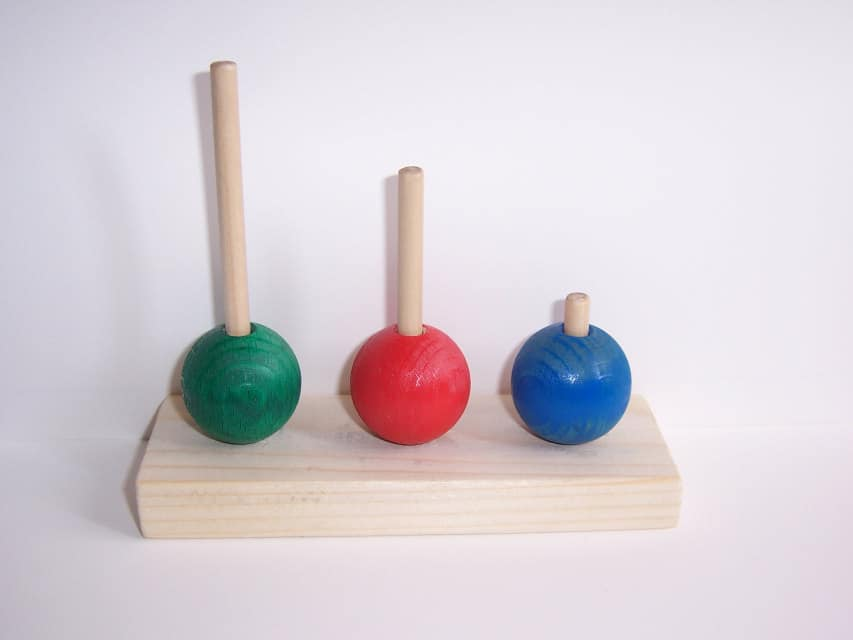
\includegraphics[width=0.45\textwidth]{immagini/TOL.png}
\caption{Supporto fisico utilizzato durante la somministrazione del test}
\end{figure}

L’obiettivo del test è spostare le palline da una configurazione iniziale a una
configurazione obiettivo, seguendo quattro regole:
\begin{enumerate}
    \item \textbf{Prima regola}: è possibile può spostare una sola pallina alla volta.
    \vspace{0.15cm}
    \item \textbf{Seconda regola}: si può muovere una sola pallina da un paletto ad un altro, in modo tale da non consentire all’utente di posizionare le palline sul tavolo o averne in mano più di una alla volta.
\vspace{0.4cm}
\item \textbf{Terza regola}: è possibile inserire una sola pallina sul paletto più
piccolo, due su quello intermedio e tre su quello più grande.
\vspace{0.4cm}
\item \textbf{Quarta regola}: bisogna attenersi al numero di spostamenti massimi consentiti
per risolvere il problema.
\end{enumerate}
\vspace{0.8cm}
Per poter calcolare il punteggio finale raggiunto dal paziente al termine del test, è
necessario tenere in considerazione il numero di problemi risolti correttamente, il
numero di mosse utilizzate per risolverli e la violazione delle regole
esplicitate precedentemente.\newline
Nel caso specifico dell’applicazione sviluppata, il test viene somministrato
dal robot Pepper attraverso i seguenti passi:
\begin{itemize}
    \item prima di iniziare il robot effettua un'introduzione al test e spiega le
regole fornendo un esempio pratico visualizzato sul suo tablet,
per assicurarsi che il paziente abbia compreso le istruzioni;
\vspace{0.4cm}
    \item dopo aver esplicitato le regole del test, il robot presenta la configurazione
iniziale del problema e la configurazione obiettivo;
\vspace{0.4cm}
    \item il paziente viene invitato da Pepper a risolvere il problema nel minor numero
possibile di mosse, senza limiti di tempo. Tuttavia, viene registrato il tempo
impiegato per completare il test a scopo diagnostico;
\vspace{0.4cm}
    \item l’esaminatore registra il numero di mosse utilizzate dal paziente, l’eventuale
violazione di regole e se il problema è stato risolto correttamente o meno;
\vspace{0.4cm}
    \item il test viene ripetuto per diverse configurazioni e nel caso specifico viene
ripetuto per 12 configurazioni con difficoltà crescente.
\end{itemize}

}
\newpage
\subsection{Implementazione}
\fontsize{12}{19}\selectfont{
Per l’implementazione di questo test sono stati utilizzati diversi
box script Python in Choregraphe, i quali verranno analizzati
di seguito:
\vspace{0.4cm}
\begin{enumerate}
    \item \textbf{Animated Say text, Record Sound, Record Video, Set language e
Face tracker}: già analizzati in precedenza.
\vspace{0.4cm}

\item \textbf{Show image}: box che permette di mostrare sul tablet di Pepper un’immagine
specifica, recuperata dalla memoria interna del robot.
\vspace{0.4cm}
\begin{figure}[H]
\centering
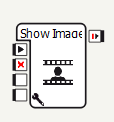
\includegraphics[width=0.2\textwidth]{immagini/si.png}
\end{figure}
\vspace{0.4cm}
\item \textbf{Set Recognition Language}: box che permette di settare la lingua riconosciuta
e compresa dal robot.
\vspace{0.4cm}
\begin{figure}[H]
\centering
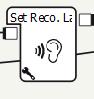
\includegraphics[width=0.18\textwidth]{immagini/srl.png}
\end{figure}
\vspace{0.4cm}
\item \textbf{Speech Recognition}: box di riconoscimento vocale che utilizza algoritmi
e modelli di riconoscimento vocale avanzati per interpretare il parlato degli
utenti.\newline Per prima cosa il box cattura l’input audio proveniente dal microfono
del robot o di un dispositivo esterno, come ad esempio un microfono
collegato al computer in cui è in esecuzione Choregraphe.\newline L’audio viene successivamente pre-elaborato
per migliorare la qualità del segnale e rimuovere eventuali rumori
di fondo indesiderati. Infine l’audio pre-elaborato viene inviato all’algoritmo
di riconoscimento vocale, che confronta il parlato con un modello linguistico
e/o una serie di modelli acustici per determinare il testo corrispondente.
\vspace{0.4cm}
\begin{figure}[H]
\centering
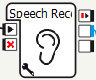
\includegraphics[width=0.18\textwidth]{immagini/sr.png}
\end{figure}
\vspace{0.4cm}
\item \textbf{Switch Case}: box che, dopo aver ricevuto la risposta dell’utente, stimola
un solo output tra quelli disponibili. Utilizzato in questo caso per proseguire
con la somministrazione del test, o ripetere le regole iniziali.
\vspace{0.4cm}
\begin{figure}[H]
\centering
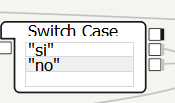
\includegraphics[width=0.27\textwidth]{immagini/sc.png}
\end{figure}
\vspace{0.4cm}
\item \textbf{Tablet touch}: box che invia un segnale nel momento in cui il tablet di
Pepper viene toccato da un utente.
\vspace{0.4cm}
\begin{figure}[H]
\centering
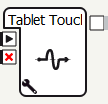
\includegraphics[width=0.18\textwidth]{immagini/tt.png}
\end{figure}
\vspace{0.4cm}
\item \textbf{Figure}: diagramma di box composto da molteplici box utilizzati per somministrare
il test ToL.
\vspace{0.4cm}
\begin{figure}[H]
\centering
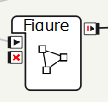
\includegraphics[width=0.2\textwidth]{immagini/figure.png}
\end{figure}
\vspace{0.4cm}
\end{enumerate}
Entrando nello specifico del box Tablet Touch questo presenta delle funzioni
python personalizzate:
\vspace{0.4cm}
\begin{itemize}
    \item \textbf{startTimer}: funzione che salva l’istante di inizio del test, per ogni figura,
in una variabile timer.
\vspace{0.6cm}
\begin{figure}[H]
\centering

\includegraphics[width=0.6\textwidth]{immagini/starttimer.png}
\end{figure}
\vspace{0.6cm}
\item \textbf{stopTimer}: funzione che interrompe il timer e calcola la durata del tempo
trascorso dal momento in cui la figura è stata mostrata al paziente, al momento
in cui viene toccato il tablet del robot.
\vspace{0.6cm}
\begin{figure}[H]
\centering
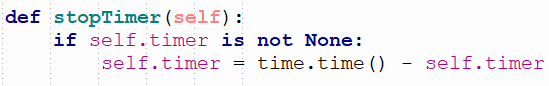
\includegraphics[width=0.8\textwidth]{immagini/stoptimer.png}
\end{figure}
\vspace{0.6cm}
\item \textbf{saveTimerValue}: funzione che, dopo aver recuperato il valore della variabile \textit{timer} (\textit{self.timer}), lo formatta in minuti e secondi.\newline Successivamente utilizza la funzione \textit{open} per inserire i dati calcolati all'interno di un file, il cui filepath è passato in input alla funzione.\newline
Il file in questione presenta un'estensione \textbf{.csv}\footnote{\textbf{Estensione CSV (Comma-Separated Values)}: viene utilizzata per rappresentare dati in un formato tabellare, dove le colonne sono separate da virgole e le righe sono separate da nuove linee. È un formato molto comune per l'archiviazione e lo scambio di dati tra diverse applicazioni.} e può essere scaricato dalla memoria del robot per poter essere analizzato successivamente.
\vspace{0.6cm}
\begin{figure}[H]
\centering
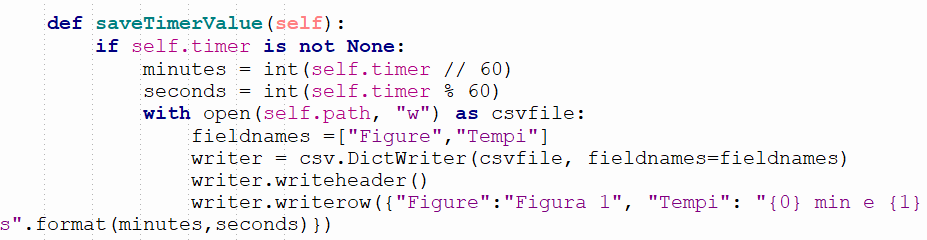
\includegraphics[width=1.15\textwidth]{immagini/stv.png}
\end{figure}
\vspace{0.4cm}
\end{itemize}
}
\newpage
\section{Risultati e obiettivi raggiunti}
\fontsize{12}{19}\selectfont{Questa sezione offre l'opportunità di riepilogare ed analizzare i principali risultati ottenuti e di sottolineare l'allineamento tra gli obiettivi prefissati e quelli raggiunti.\newline

Considerando i due test analizzati in precedenza, nel caso del \textbf{test sulla Discriminazione uditiva} si è sviluppata una applicazione
con comportamenti personalizzati del robot in grado di simulare la
somministrazione della prova da parte di un terapista.\newline
\begin{figure}[H]
\centering
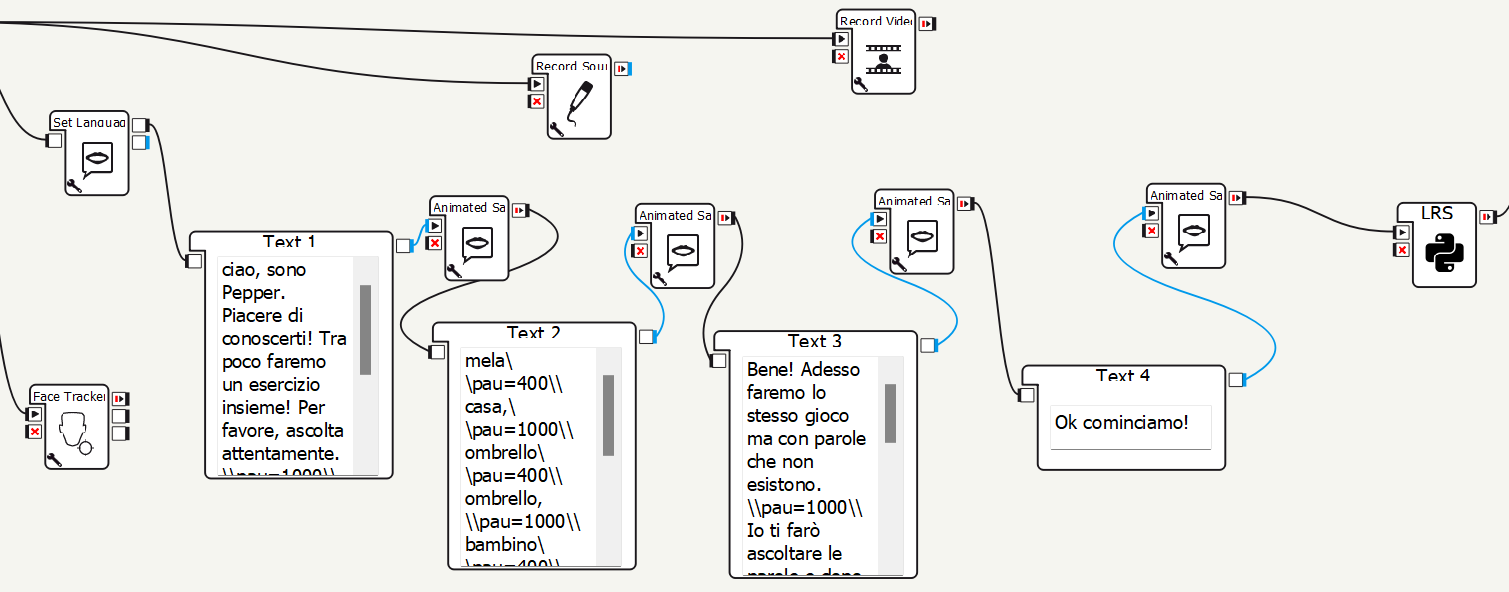
\includegraphics[width=1.1\textwidth]{immagini/tdu.png}
\caption{Panoramica sul test della Discriminazione uditiva}
\end{figure}
\vspace{0.4cm}
Più nello specifico,
inizialmente Pepper effettua un’ introduzione al test, spiegando dettagliatamente
le regole di quest’ultimo, per poi comunicare al paziente le 37 coppie
di \textit{non parole}.\newline
Il robot attende la risposta del paziente e aggiorna il suo
score prima di aver comunicato la successiva coppia di non parole. Al termine
del test si è in grado di visionare un file di testo contente lo \textit{score} del paziente,
da analizzare successivamente.\newline

Analizzando invece il \textbf{test della Torre di Londra (ToL)}, l’applicazione
sviluppata permette anche in questo caso di simulare la somministrazione
della prova da parte di un terapista, pur non sostituendo la sua valutazione.\newline
Il robot dopo una prima fase nella quale fornisce al paziente una spiegazione
delle regole, mostra una configurazione di prova da utilizzare per verificare
la comprensione della struttura del test somministrandolo successivamente.
\vspace{0.6cm}
\begin{figure}[H]
\centering
\includegraphics[width=0.75\textwidth]{immagini/TOL1.png}
\caption{Esempio di configurazione che il paziente deve replicare (ToL)}
\end{figure}
\newpage
A questo punto il paziente visualizza sul tablet di Pepper la configurazione
da replicare, riproduce quella compresa e prosegue in questo modo fino ad
esaurire tutte le configurazioni fornite dall’umanoide.

Al termine della prova, verranno analizzati dal terapista tutti i dati raccolti, salvati nel file cvs realizzato da Pepper e contenente i tempi di esecuzione del paziente per ogni singola configurazione.
\vspace{0.6cm}
\begin{figure}[H]
\centering
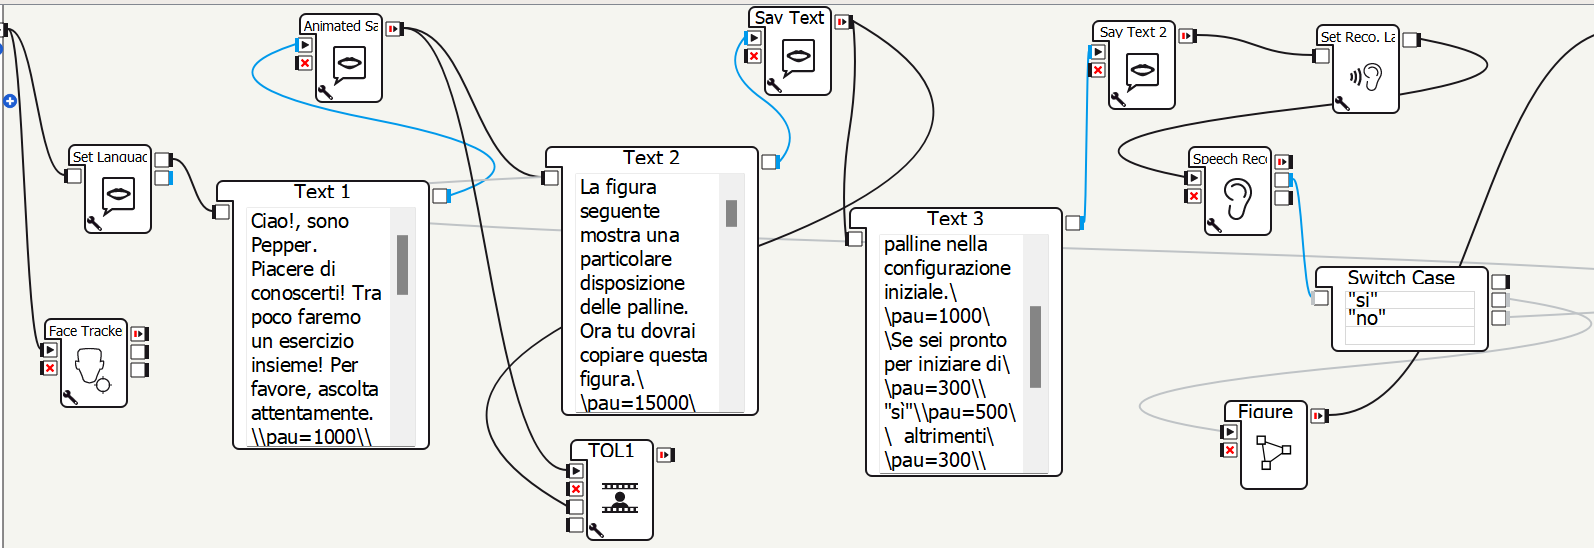
\includegraphics[width=1\textwidth]{immagini/tol1.png}
\caption{Panoramica sul test della Torre di Londra (ToL)}
\end{figure}
\vspace{1cm}
\begin{figure}[H]
\centering
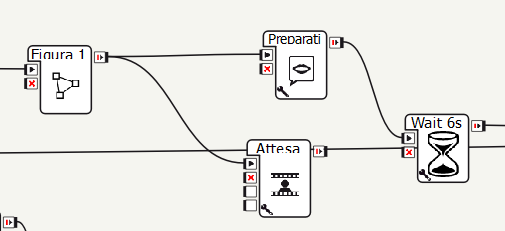
\includegraphics[width=0.7\textwidth]{immagini/tol2.png}
\caption{Implementazione della visualizzazione delle figure sul tablet di Pepper}
\end{figure}
\newpage
}
 \end{sloppypar}
\afterpage{\blankpage}
 \begin{sloppypar}
\chapter{Sviluppi Futuri}
\section{Introduzione}
\fontsize{12}{19}\selectfont{
Nel corso dell’ultimo decennio sono stati condotti numerosi studi sull’applicazione della robotica nel campo della disabilità. 
La terapia assistita da robot è un campo di ricerca ed applicazione promettente \cite{Numero12}, un’altra delle sfide che tecnologia e clinica affrontano insieme allo scopo di supportare i pazienti. Una parte rilevante delle attuali ricerche si è focalizzata sull’utilità delle tecnologie robotiche nello stimolare le abilità deficitarie nei Disturbi dello Spettro Autistico, dando conferma di come i robot umanoidi possano fornire un valido aiuto nel creare una comunicazione con il paziente, favorendone l’attenzione e generando nuovi comportamenti sociali.\newline
Dagli studi che si sono succeduti negli anni, è emerso che i robot umanoidi, senza mai  sostituirsi all’essere umano, migliorano le competenze sociali dei pazienti, per i quali l’interazione con le altre persone è un elemento che disorienta, anche a causa della variegata espressività del volto umano; interagendo con una persona, i pazienti affetti da DSA vengono a contatto con numerosi segnali sociali (le espressioni facciali, i gesti, la tonalità della voce) per loro difficili da interpretare.\newline
Il robot diventa quindi una sorta di intermediario, affidabile e prevedibile, uno strumento conoscitivo per apprendere maggiori informazioni sul funzionamento della mente dei pazienti e di supporto per un percorso diagnostico e terapeutico completo.
\vspace{1.5cm}
\begin{figure}[H]
\centering
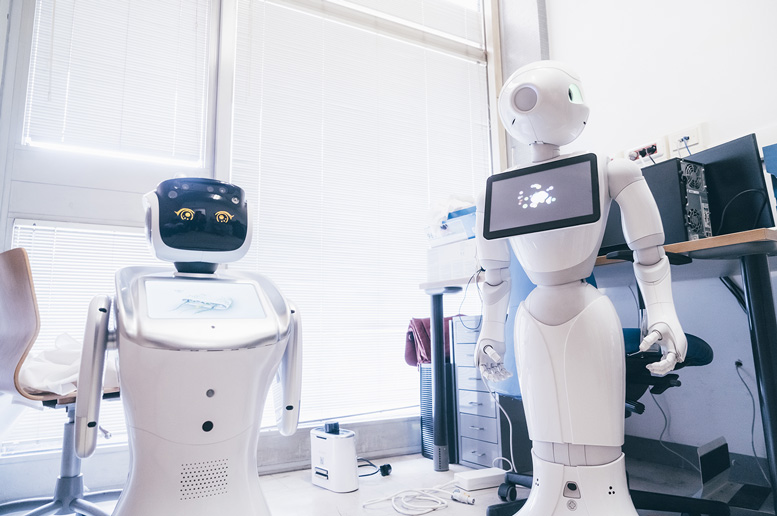
\includegraphics[width=0.8\textwidth]{immagini/pepper_finale.jpg}
\caption{Robot assistenziali utilizzati nel reparto di pediatria dell'ospedale di Padova}
\end{figure}
\vspace{1cm}
\newpage
Nel prossimo futuro, si prevede che l’Intelligenza Artificiale parteciperà in modo progressivo ai processi decisionali in ambito sanitario e i professionisti del settore  utilizzeranno sempre più dispositivi di intelligenza artificiale e apprendimento automatico per migliorare la precisione nella diagnosi e identificare i regimi terapeutici.\newline
Tuttavia, pur offrendo numerose possibilità anche molto promettenti, l’adozione dei robot di assistenza rimane ancora inferiore al previsto, per un gap tra tecnologia e assistenza sanitaria. Gap che non deriva esclusivamente dalle attuali strategie per l’implementazione dei robot, ma è piuttosto un gap informativo nelle sezioni trasversali della progettazione tecnologica, della sanità e della società.\newline
E’ necessaria una diffusione delle conoscenze che favorisca l’interazione e la condivisione delle informazioni tra tutte le parti interessate coinvolte  nella gestione dei robot per la diagnosi e cura dei DSA. La progettazione e l'implementazione di un robot richiedono competenze multidisciplinari provenienti da settori quali l'ingegneria, l'informatica, la psicologia e la riabilitazione clinica e la collaborazione tra i professionisti delle diverse discipline può portare ad un numero maggiore di contributi in questa area di ricerca con conseguenti ricadute positive sui pazienti.
\newline
Rimangono importanti i punti a favore della terapia assistita da robot. Essendo trattamenti informatizzati, è possibile tracciare e monitorare i progressi e gli step del trattamento, senza la necessità di affidarsi alle tecniche di osservazione tradizionali, personalizzando e adattando i percorsi alle specifiche esigenze del singolo paziente.\newline
I disturbi dello spettro autistico si caratterizzano per la grande variabilità che c’è tra un soggetto e l’altro e la possibilità di avere strumenti condivisi ma personalizzabili è sicuramente di grande vantaggio per i clinici.
Una delle sfide più ardue è quella di rendere le soluzioni tecnologiche offerte dalla robotica assistiva usabili ed accettabili per i soggetti che dovrebbero trarne beneficio. Questo passaggio è tutt’altro che scontato. In questo senso, un approccio che nasce nel mondo dell’architettura e del design, ma che tende progressivamente ad estendersi alla progettazione di soluzioni tecnologiche ovvero di servizi integrati con soluzioni tecnologiche, è il cosiddetto \textit{Human Centered Approach}. Il punto cardine di questo modello, come evidenziato dal nome, consiste nel mettere al centro della progettazione la persona e i suoi bisogni, per far sì che i desideri e le aspettative da questa espressi siano la linea guida per lo sviluppo del prodotto o servizio. Infine, esso mira ad includere la prospettiva di tutti coloro che possono avere un interesse nella realizzazione e ad assumere quindi non solo il punto di vista dell’utente finale ma anche quello di eventuali operatori, manutentori, specialisti, etc.
}
\newpage
\section{Funzionalità future dell' applicazione}
\fontsize{12}{19}\selectfont{Attraverso l’impiego di tecnologie avanzate e l’applicazione di principi psicologici specifici, definiti anche grazie alla collaborazione con professionisti del settore, è stato possibile realizzare uno strumento accessibile, intuitivo e personalizzabile.\newline
Al momento sono in fase di studio e realizzazione nuove possibili funzionalità dell’applicazione, in particolare una dashboard e un database dedicato, come di seguito descritte:
\vspace{0.5cm}
\begin{enumerate}
    \item \textbf{Dashboard}: interfaccia \textit{user-friendly} di supporto ai clinici per avere accesso immediato alla raccolta di tutti i test da somministrare ai pazienti e per monitorarne i progressi durante la terapia nel corso del tempo. 
    \vspace{0.5cm}
    \item \textbf{Database dedicato}: organizzazione strutturata delle informazioni raccolte da Pepper, per consentirne il salvataggio, la visualizzazione e un facile reperimento da parte degli utenti.\newline
    Il database da utilizzare memorizzerà le seguenti informazioni:
    \begin{itemize}
     \vspace{0.5cm}
    \item Parametri facciali univoci associati ad  un dato paziente e restituiti dal modulo di riconoscimento facciale del robot.
     \vspace{0.5cm}
    \item Informazioni anagrafiche e sanitarie, contenenti la storia clinica di ogni paziente.
     \vspace{0.5cm}
        \item Registrazione video delle sedute di somministrazione dei test, identificate dal codice univoco di ogni paziente e dalla data di acquisizione.
         \vspace{0.5cm}
        \item Registrazione audio delle sedute di somministrazione dei test, identificate dal codice univoco di ogni paziente e dalla data di acquisizione.
    \end{itemize}
\end{enumerate}
}
 \end{sloppypar}
\afterpage{\blankpage}
 \begin{sloppypar}
\chapter{Conclusioni}
\fontsize{12}{19}\selectfont{
Negli ultimi anni la robotica sociale assistita (RSA) è stata oggetto di studio scientifico e di applicazione clinica nel trattamento e nella diagnosi del Disturbo dello Spettro Autistico (DSA).
Gli studi in questo settore hanno dimostrato che  l’uso  della  RSA  può  migliorare  l’attenzione  e  il  coinvolgimento dei pazienti affetti da disturbi dello spettro autistico, promuovere l’interazione sociale e comunicativa e supportare i professionisti del settore sanitario.\newline
In questo lavoro  di  tesi è  stata  presentata e descritta  un'applicazione  sviluppata per la somministrazione attraverso il robot umanoide \textit{Pepper - SoftBank Robotics}\texttrademark \space di test per l’analisi delle funzioni cognitivo-linguistiche in individui affetti da disturbi dello spettro autistico.\newline
L’applicazione sviluppata si è dimostrata efficace nel facilitare la somministrazione dei test e la raccolta dei risultati ottenuti.\newline
Essa consente un certo grado di standardizzazione delle procedure e un’analisi più veloce e dettagliata dei dati, generalmente collezionati solo in forma cartacea.\newline 
Ci si augura che gli sviluppi futuri previsti siano in grado nel breve tempo di rendere l’applicazione ancora più efficiente al fine di una valutazione sempre più accurata delle funzioni cognitive-linguistiche dei pazienti, facilitando la  gestione e l’elaborazione di informazioni utili alla diagnosi, alla pianificazione delle terapie e al monitoraggio dei loro progressi nel tempo.
}
 \end{sloppypar}
\afterpage{\blankpage}
\begin{sloppypar}
\chapter*{Ringraziamenti}


\fontsize{12}{19}\selectfont{Al termine del lavoro di tesi, desidero dedicare questo spazio per esprimere la mia gratitudine a tutte quelle persone che hanno contribuito al raggiungimento di questo mio primo traguardo.\vspace{0.3cm}\newline In primo luogo desidero ringraziare di cuore il mio relatore, la Professoressa Mariacarla Staffa, il suo supporto costante, la sua competenza e la sua guida sono stati fondamentali per la realizzazione di questa tesi. Desidero ringraziarla soprattutto per avermi trasmesso la sua passione per gli argomenti trattati e per essere stata una presenza stimolante durante il mio percorso accademico. Auguro a tutti i miei colleghi di incontrare un docente come lei, in grado di tenere viva e alimentare la "fiamma" della conoscenza.\vspace{0.3cm}\newline
Un ringraziamento speciale va ai miei genitori, per avermi sempre sostenuto in ogni fase della mia vita. Grazie per tutti i vostri sacrifici, per aver sempre creduto in me e per avermi incoraggiato a perseguire i miei obiettivi.\vspace{0.3cm}\newline Ringrazio mio fratello Stefano, per il suo sostegno incondizionato durante tutto il mio percorso accademico. La sua voglia di fare e la sua saggezza sono per me una guida preziosa e un esempio da seguire. Grazie per essere sempre al mio fianco.\vspace{0.3cm}\newline Non posso non ringraziare la mia ragazza, Emilia, per il suo amore incondizionato e per avermi sempre spronato a dare il meglio di me. La sua forza, la sua determinazione e il suo modo di affrontare la vita, sempre con il sorriso, sono per me grande fonte di ispirazione. Il raggiungimento di qualsiasi obiettivo non sarebbe lo stesso senza la sua presenza al mio fianco.\vspace{0.3cm}\newline Infine, desidero esprimere profonda gratitudine al mio migliore amico, Davide, un compagno fedele e un vero fratello per me. Le risate, le avventure e i ricordi che abbiamo condiviso rappresentano un bagaglio personale di inestimabile valore. La sua amicizia è stata un supporto fondamentale durante il mio percorso personale e accademico. Mi auguro di continuare a sostenere reciprocamente i nostri sogni e le nostre ambizioni future.\vspace{0.3cm}\newline Concludo ringraziando tutti gli amici e i compagni di corso, per gli scambi di idee e il sostegno reciproco, che hanno reso questi anni universitari più ricchi e significativi.\vspace{0.3cm}\newline A tutti voi, rinnovo il mio più sincero grazie.
}
\end{sloppypar}
\addcontentsline{toc}{chapter}{Ringraziamenti}

\bibliographystyle{unsrturl}
\bibliography{bibliografia}

\end{document}
